\section{Semantiek van predikaatlogica}

 \begin{answer} % 6.1
 Stel we gebruiken het functiesymbool `$-$' voor de bewerking `aftrekken'. Als $E$ staat voor `is even' en `$P$' voor `is een priemgetal', wat drukken de volgende formules dan uit?
 \begin{enumerate}
     \item $\forall x((E(x)\wedge x>2)\rightarrow\exists y(P(y)\wedge P(x-y)))$ \\
     antwoord: Voor alle x geldt dat als het even is en groter dan 2, dan is er een y dat een priemgetal is en als je het van x aftrekt het resultaat ook een priemgetal is. \\
     In andere woorden: Voor alle even getallen groter dan 2 geldt dat er priemgetal y is waarbij het verschil tussen x en y ook een priemgetal is.
     \item $\neg\exists x(P(x)\wedge\forall y(P(y)\rightarrow y\leq x))$ \\
     antwoord: Het is niet zo dat er een x is waarvoor geldt dat x een priemgetal is en voor alle y geldt dat als y een priemgetal is dat y kleiner of gelijk is aan x. \\
     In andere woorden: Er is geen priemgetal dat groter of gelijk is aan alle andere priemgetallen. 
 \end{enumerate}
 \end{answer}
 
 \begin{answer} % 6.2
 Beschouw de formule $\forall x\forall y\forall z((R(x,y)\wedge R(y,z))\rightarrow R(x,z))$.
 \begin{enumerate}
     \item Is deze formule waar in een model met de natuurlijke getallen als objecten, waarin $R$ overeenkomt met de gewone kleiner-dan-relatie ($<$)? \\
     Antwoord: ja, in dat model en die definitie van $R$ klopt het. De formule laat zich dan vertalen naar: $x < y \wedge y < z \rightarrow x < z$. Als x een getal kleiner dan y is en y een getal kleiner dan z is, dan moet x ook kleiner zijn dan z.
     \item En in een model met dezelfde verzameling objecten, maar nu met de relatie $R$ gedefinieerd door: $R(x, y)$ precies dan als $x\leq y+1$? \\
     antwoord: Het model is het zelfde. De relatie is wel anders. We moeten nu de formule lezen als:  $x \leq y+1 \wedge y \leq z+1 \rightarrow x \leq z+1$. We kunnen nu wel een tegenvoorbeeld construeren. Bij $x = 5$, $y = 4$ en $z = 3$ is de formule niet waar. 
     \item Is de formule waar in het model uit voorbeeld 6.1?\\
     antwoord: Ja, in het model uit het voorbeeld is de formule waar.
     \item Is de formule waar in elk model met precies twee objecten? Zo ja, bewijs dit, zo nee, geef een voorbeeld van een model met twee objecten waarop de formule niet waar is. \\
     antwoord: We kunnen een tegenvoorbeeld maken: \\
     \begin{center}
        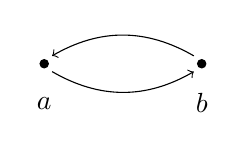
\begin{tikzpicture}
        \draw[fill] (0,0) circle (1.5pt);
        \draw[fill] (2,0) circle (1.5pt);
        \draw [->] (1.9,0.1) to [out=150,in=30] (0.1,0.1);
        \draw [->] (0.1,-0.1) to [out=-30,in=210] (1.9,-0.1);
        \node at (0,-.5) {$a$};
        \node at (2,-.5) {$b$};
        \end{tikzpicture}
        \end{center}
    Op het gegeven voorbeeld geldt $R(a,b)$ en $R(b,a)$, maar niet (zie formule) $R(a,a)$ (als $x=a, y=b, z=a$) of $R(b,b)$ (als $x=b, y=a, z=b$).
 \end{enumerate}
 \end{answer}
 
\begin{answer} % 6.3
Beschouw het volgende model:
\begin{center}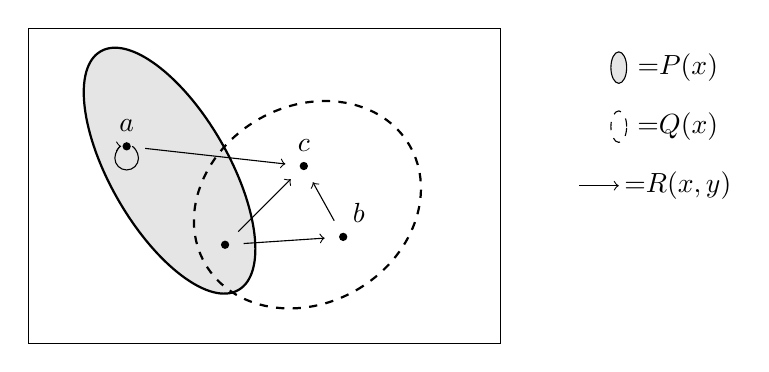
\begin{tikzpicture}
\draw (0,0) rectangle (6,4);
\draw[thick,fill=gray!20,rotate=30] (2.65,1) ellipse (.75cm and 1.75cm);
\draw[thick,dashed,rotate=-60] (.25,3.95) ellipse (1.25cm and 1.5cm);
\node[circle,fill,inner sep=0pt,minimum size=3pt,label={[anchor=south]north:$a$}] at (1.25, 2.5) (a) {};
\node[circle,fill,inner sep=0pt,minimum size=3pt] at (2.5, 1.25) (d) {};
\node[circle,fill,inner sep=0pt,minimum size=3pt,label={[anchor=south west]north:$b$}] at (4,1.35) (b) {};
\node[circle,fill,inner sep=0pt,minimum size=3pt,label={[anchor=south]north:$c$}] at (3.5,2.25) (c) {};
\draw[->,shorten <=2pt,shorten >=2pt] (a) arc(90:-270:.15); 
\draw[->,shorten <=5pt,shorten >=5pt] (a) -- (c); 
\draw[->,shorten <=5pt,shorten >=5pt] (d) -- (c); 
\draw[->,shorten <=5pt,shorten >=5pt] (d) -- (b); 
\draw[->,shorten <=5pt,shorten >=5pt] (b) -- (c);
\draw[fill=gray!20] (7.5,3.5) ellipse (.1cm and .2cm);\node at (8.25,3.5) {=$P(x)$};
\draw[dashed] (7.5,2.75) ellipse (.1cm and .2cm);\node at (8.25,2.75) {=$Q(x)$};
\draw[->] (7,2) -- (7.5,2);\node at (8.25,2) {=$R(x,y)$};
\end{tikzpicture}
\end{center}
Beredeneer welke van de volgende formules geldig zijn op het gegeven model:
\begin{enumerate}
    \item $R(a,a)$\\
    antwoord: Geldig, er is een pijl van $a$ naar $a$.
    \item $R(x,x)$\\
    antwoord: Onbekend, als $x=a$ dan geldig, anders ongeldig.
    \item $\exists y\; R(a,y)$\\
    antwoord: Geldig, kies bijvoorbeeld voor $x = c$.
    \item $\exists x\; R(x,x)$\\
    antwoord: Geldig, kies voor $x=a$.
    \item $\neg\forall x(P(x)\rightarrow R(x,x))$\\
    antwoord: Geldig, $\forall x(P(x)\rightarrow R(x,x))$ (= `vanuit elk element in $P$ loopt een pijl naar zichzelf') is niet waar, de negatie hiervan is dus geldig.
    \item $\exists x(P(x)\wedge R(x,x))$\\
    antwoord: Geldig, er is een $x$ in $P$ met een pijl naar zichzelf ($x=a$).
    \item $\forall x\exists y\;R(x,y)$\\
    antwoord: Niet geldig; $c$ heeft geen uitgaande pijl (er is geen $y$ te kiezen als $x=c$ zodanig dat $R(c,y)$).
    \item $\forall x(R(x,x)\rightarrow P(x))$
    antwoord: Geldig, alle elementen met een pijl naar zichzelf (alleen $a$), zit in $P$.
    \item $\forall x\bigl[P(x)\rightarrow\exists y\;R(x,y)\bigr]$\\
    antwoord: Geldig, elk element in $P$ heeft een pijl naar een ander element.
    \item $\forall x\bigl[P(x)\rightarrow\exists y(R(x,y)\wedge Q(y))]$\\
    antwoord: Geldig, elk element in $P$ heeft een pijl naar een element in $Q$.
\end{enumerate}
\end{answer}

\begin{answer} % 6.4
Beschouw het domein $\mathbb{N}$ van natuurlijke getallen, met $E$ als het even-predikaat ($E(x)$ wil zeggen `$x$ is even') en een $A$ als optel-predikaat ($A(x,y,z)$ wil zeggen `$x+y=z$').

Geef aan of de volgende zinnen waar zijn op dit model:
\begin{enumerate}[label=\textit{\alph*.}]
\item $\forall x(E(x)\leftrightarrow\exists y\;A(y,y,x))$;\\
antwoord: Dit is waar. Voor elk getal dat even is geldt dat het deelbaar door twee is. Dus voor elke even getal x is er een getal y waarvoor geldt y + y = x. Andersom is dit natuurlijk ook waar. Als je een getal kan maken door het zelfde getal keer twee doen (y + y), dan is dit getal even.
\item $\forall z\exists x\exists y(\neg(x=y)\wedge A(x,y,z))$; \\
antwoord: Dit is niet waar. Natuurlijke getallen bestaan uit alle gehele getallen boven de of gelijk zijn aan 0. Een tegenvoorbeeld voor deze stelling is: $z = 0$. Zijn nu geen twee verschillende getallen die opgeteld 0 zijn. 
\item $\forall x\forall y\forall z((E(x)\wedge E(y)\wedge A(x, y, z))\rightarrow E(z))$. \\
antwoord: Dit is waar. Als je twee even getallen bij elkaar optelt, dan is het resultaat ook altijd een even getal.
\end{enumerate}
\end{answer}

\begin{answer} % 6.5
Gegeven is de volgende informatie over een model:\\
Predikaten $P,Q$ en $P$ is een-plaatsig, $Q$ is twee-plaatsig.\\
1 constante $c$.
$$A:= \forall x (P(x)\rightarrow\exists y\; Q(x,y))$$
\begin{enumerate}[label=\textit{\alph*.}]
\item Teken een model waar deze formule waar is.\\
antwoord: 
\begin{center}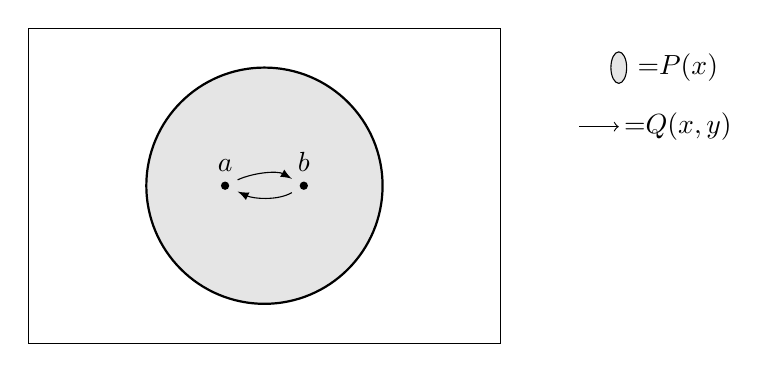
\begin{tikzpicture}
\draw (0,0) rectangle (6,4);
\draw[thick,fill=gray!20] (3,2) ellipse (1.5cm and 1.5cm);
\node[circle,fill,inner sep=0pt,minimum size=3pt,label={[anchor=south]north:$a$}] at (2.5, 2) (a) {};
\node[circle,fill,inner sep=0pt,minimum size=3pt,label={[anchor=south]north:$b$}] at (3.5,2) (b) {};
\draw[->,shorten <= 5pt, shorten >= 5pt,out=25,in=150,>=latex] (2.5, 2) to (3.5,2);
\draw[->,shorten <= 5pt, shorten >= 5pt,out=-150,in=-25,>=latex] (3.5, 2) to (2.5,2);
\draw[fill=gray!20] (7.5,3.5) ellipse (.1cm and .2cm);\node at (8.25,3.5) {=$P(x)$};
\draw[->] (7,2.75) -- (7.5,2.75);\node at (8.25,2.75) {=$Q(x,y)$};
\end{tikzpicture}
\end{center}
Toelichting: \\
Neem $x = a$ en $y = b$,  dat geeft $P(a) \rightarrow Q(a,b)$ en dit is waar. \\
Neem $x = b$ en $y = a$,  dat geeft $P(b) \rightarrow Q(b,a)$ en dit is waar.\\
Dus voor ieder element $x$ kunnen we een element $y$ vinden die de formule waar maakt,  dus dit model maakt $A$ waar.
\item Teken een model waar deze formule onwaar is.
$$B:=(P(c)\wedge\forall x(P(x)\rightarrow\exists y(Q(x,y)\wedge P(y))))$$
antwoord (simpel):
\begin{center}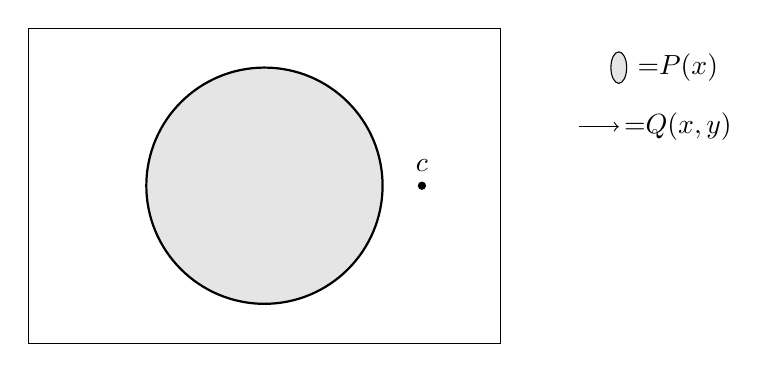
\begin{tikzpicture}
\draw (0,0) rectangle (6,4);
\draw[thick,fill=gray!20] (3,2) ellipse (1.5cm and 1.5cm);
\node[circle,fill,inner sep=0pt,minimum size=3pt,label={[anchor=south]north:$c$}] at (5, 2) (c) {};
\draw[fill=gray!20] (7.5,3.5) ellipse (.1cm and .2cm);\node at (8.25,3.5) {=$P(x)$};
\draw[->] (7,2.75) -- (7.5,2.75);\node at (8.25,2.75) {=$Q(x,y)$};
\end{tikzpicture}
\end{center}
Toelichting: $P(c)$ is onwaar, dus $P(c)\wedge\forall x(P(x)\rightarrow\exists y(Q(x,y)\wedge P(y)))$ is ook onwaar. \\
antwoord (moeilijker):
\begin{center}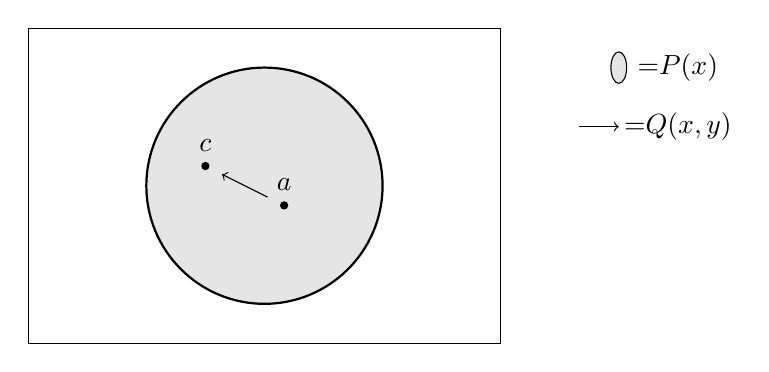
\begin{tikzpicture}
\draw (0,0) rectangle (6,4);
\draw[thick,fill=gray!20] (3,2) ellipse (1.5cm and 1.5cm);
\node[circle,fill,inner sep=0pt,minimum size=3pt,label={[anchor=south]north:$c$}] at (2.25, 2.25) (c) {};
\node[circle,fill,inner sep=0pt,minimum size=3pt,label={[anchor=south]north:$a$}] at (3.25, 1.75) (a) {};
\draw[->,shorten <=5pt,shorten >=5pt] (a) -- (c);
\draw[fill=gray!20] (7.5,3.5) ellipse (.1cm and .2cm);\node at (8.25,3.5) {=$P(x)$};
\draw[->] (7,2.75) -- (7.5,2.75);\node at (8.25,2.75) {=$Q(x,y)$};
\end{tikzpicture}
\end{center}
Toelichting: $P(c)$ is waar, dus om te laten zien dat formule $B$ onwaar is,  moeten we laten zien dat $\forall x(P(x)\rightarrow\exists y(Q(x,y)\wedge P(y))$ onwaar is. \\
Neem $x = a$ en $y = a$,  dat geeft $P(a) \rightarrow (Q(a,a) \wedge P(a))$ en dit is onwaar (bij twijfel kun je dit controleren met een waarheidstabel).\\
Neem $x = a$ en $y = c$,  dat geeft $P(a) \rightarrow (Q(a,c) \wedge P(c))$.   Dit is waar.  Dus voor $x = a$ kunnen we een $y$ vinden die de formule waar maakt.  Nu bekijken we dit voor $x = c$:\\
Neem $x= c$ en $y = c$,  dat geeft $P(c) \rightarrow (Q(c,c) \wedge P(c))$, wat onwaar is. \\
Neem $x =c$ en $y=a$, dat geeft $P(c) \rightarrow (Q(c,a) \wedge P(a))$,  wat onwaar is. \\
Voor $x=c$ is er dus geen $y$ te vinden die de formule waar maakt,  dus $B$ is onwaar.\\
Merk op: Om aan te tonen dat de formule onwaar is,  zouden we de stappen bij $x=a$ weg kunnen laten,  aantonen dat het onwaar is voor $x=c$ is voldoende.  

%\begin{enumerate}[label=\textit{\alph*.}]
\setcounter{enumi}{2}
\item Hoeveel elementen heb je minimaal nodig in een model om $B$ waar te maken?\\
antwoord: Er is \'e\'en element $c$ nodig om $P(c)$ waar te maken.  Om te zien dat \'e\'en element ook voldoende is beschouwen we het volgende model:
\begin{center}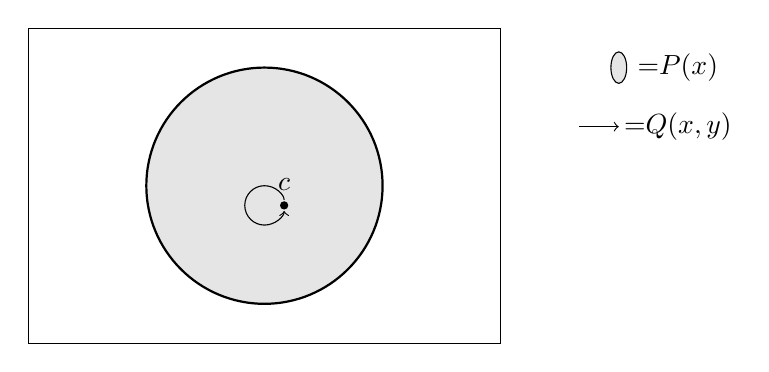
\begin{tikzpicture}
\draw (0,0) rectangle (6,4);
\draw[thick,fill=gray!20] (3,2) ellipse (1.5cm and 1.5cm);
\node[circle,fill,inner sep=0pt,minimum size=3pt,label={[anchor=south]north:$c$}] at (3.25, 1.75) (c) {};
\draw[->,shorten <=2pt,shorten >=2pt] (c) arc(0:360:.25); 
\draw[fill=gray!20] (7.5,3.5) ellipse (.1cm and .2cm);\node at (8.25,3.5) {=$P(x)$};
\draw[->] (7,2.75) -- (7.5,2.75);\node at (8.25,2.75) {=$Q(x,y)$};
\end{tikzpicture}
\end{center}
Toelichting: $P(c)$ is waar,  dus we hoeveel alleen nog aan te tonen dat $\forall x(P(x)\rightarrow\exists y(Q(x,y)\wedge P(y)))$ waar is.  Aangezien er maar 1 element is,  is het voldoende dit voor $x = c$ te controleren. 
Neem $x = c$ en $y = c$,  dat geeft $P(c) \rightarrow (Q(c,c) \land P(c))$.  Dit is waar,  dus dit model maakt formule $B$ waar.\\
Merk op: bij twijfel kun je de waarheid van $P(c) \rightarrow (Q(c,c) \land P(c))$ controleren met een waarheidstabel.

\end{enumerate}\mbox{}\\[2.5pt]
\end{answer}
